\documentclass[a4paper,11pt]{article}
\usepackage{fullpage}
\usepackage{amsmath}
\usepackage{xcolor}
\usepackage{qcircuit}
\usepackage{amsmath}
\usepackage{graphicx}

\newcommand*{\Perm}[2]{{}^{#1}\!P_{#2}}%

\begin{document}
	
	\title{Quantum speedup in testing causal hypotheses: Nutshell}
	\author{aqasch}
	\date{}
	\maketitle
	\section{Introduction}
	To test hypothesis about the causal structure in a setting where we have different \textit{prior hypothesis} of how we infer a bunch of variables are causally related to each other. \textbf{We aim to find which hypothesis is the correct one among the set of prior considerations}.
	
	\subsection{Test} To causal hypothesis one need to emphasize an allotted role of intervention and how it is important to plan carefully the interventions in order to maximize our chances to find out the right hypothesis.
	
	\subsection{Causality} For a set of variables in $A$ and in $B$, we can say \textbf{$A$ is a cause for $B$} if and only if \textbf{our ability to intervene $A$ has a visible effect on the statistics of $B$}.
	
	\subsection{Caveat} Famous conclusion says \textbf{``Correlation does not imply Causation"}. So it is not enough to study the natural correlations between variables in order to establish a causal link. \textbf{Hence it is important to be able to test and probe different causal settings} as \textit{single joint probability distribution is not enough for that}.
	
	\subsection{Recent advances in quantum}
	Recent advances in ``causal relation" and ``causal networks" to quantum theory and beyond considers the \textbf{causal variables as physical systems}. The causal relations are defined as \textbf{$A$ is a cause for $B$ if changing the parameters of the state of $A$ induces a change of the state $B$}.
	
	\subsection{Could you please motivate me to invest my precious time in this quantum extension?}
	Sure! So there are foundational and practical reasons. Follow me as I say
	\begin{itemize}
		\item There are some well known quantum features such as \textbf{superposition}, \textbf{entanglement}, \textbf{nonlocality} and not-so-well known quantum features like \textbf{contextuality}. And there are some features that are involved in discovering causal relationships. 
		
		\textbf{Finding the relation between quantum and causal-relation discovering features may help us to get better insight to a theory that combine important role of causality and quantum} $\rightarrow$ \textbf{\textcolor{red}{QUANTUM GRAVITY}}.
		
		\item It would be fascinating to \textbf{axiomatize quantum theory which has something to do with ability to distinguish between causal relationships}.
		
		\item \textbf{To identify working principles for a new quantum device}. Also, to develop a technology for quantum causality.
	\end{itemize}
	
	
	\subsection{An Example}
	To distinguish between
	\begin{itemize}
		\item \textcolor{red}{1st hypothesis:} \textbf{$A$ causes $B$}
		\begin{equation}
			\Qcircuit @C=1em @R=.7em {
				& \multigate{1}{\rho} & \gate{\mathcal{M}_a} & \multigate{1}{\mathcal{C}} & \gate{\mathcal{N}_b} & \gate{\text{Tr}} \\
				& \ghost{\rho} & \qw & \ghost{\mathcal{C}}
			}\nonumber	
		\end{equation}
		The variables are distinguished in two parts \textit{input} and \textit{output}. Whatever comes from $\mathcal{M}_a$ (which is our choice of measurement on $a$) causes $b$ i.e. it effects the measurement outcome of $b$ presented through $\mathcal{N}_b$.
		\item \textcolor{red}{2nd hypothesis:} \textbf{$A$ and $B$ have a common cause}
		\begin{equation}
			\Qcircuit @C=1em @R=.7em {
				& \multigate{1}{\rho} & \gate{\mathcal{M}_a}  & \gate{\text{Tr}} \\
				& \ghost{\rho} & \gate{\mathcal{N}_b} & \gate{\text{Tr}}
			}\nonumber	
		\end{equation}
		It means there was a physical system prepared and the two measurements $\mathcal{M}_a$ and $\mathcal{N}_b$ are acting parallel on two different subsystems.
	\end{itemize}
	\subsubsection{Solution}
	\textbf{1st situation:} Consider in \textcolor{red}{1st hypothesis} $\mathcal{C}=\mathcal{I}$ i.e. identity. Then if $\mathcal{M}_a$ and $\mathcal{N}_b$ are the same projective measurement then we expect to observe the same outcome. And by investigating this correlation over all possible measurements we can be assured that we are in \textcolor{red}{1st hypothesis}. It is not possible in \textcolor{red}{2nd hypothesis}.
	\\
	
	\noindent\textbf{2nd situation:} If we use the same orthogonal measurement in \textcolor{red}{2nd hypothesis} then we will observe perfect anti-correlation. i.e. if $\mathcal{M}_a=0$ then $\mathcal{N}_b=1$. If this appears for each and every possible setting then we can conclude that $A$ and $B$ are of common cause.
	\\
	
	\noindent \textbf{Conclusion:} For a specific $\rho$ and $\mathcal{C}$ it is possible to distinguish between \textcolor{red}{1st} and \textcolor{red}{2nd hypothesis} using only \textit{projective measurements}.
	In the \textcolor{red}{hypothesis} by scanning the two projective measurements $\mathcal{M}_a$ and $\mathcal{N}_b$ over all possible settings we can reach the above conclusion.
	\\
	
	\noindent\textbf{Classical:} In projective classical measurement we really see the value of a variable and we do not change it. So in classical theory we would have no way to to distinguish two hypothesis.
	
	\subsection{Question}
	The type of advantage we show above is restricted to the specific kinds of allowed measurements where \textbf{classical theory is restricted to passive observational strategies} and no intervention is allowed.
	
	\noindent\textbf{\textcolor{red}{Can we find the advantage in a situation where arbitrary interventions are allowed?}}
	
	\subsection{Causal discovery vs Causal hypothesis testing}
	In \textbf{Causal discovery} we have variables as \textit{input} and we get a causal relation among them as \textit{output}.
	\\
	\noindent In \textbf{Causal hypothesis testing} we have variables and a \textit{set of hypothesis on causal relations among them} as \textit{input} and we get correct hypothesis as \textit{output}.
	
	\section{Causal Hypothesis}
	Two causal hypothesis
	\begin{itemize}
		\item \textbf{$A$ causes $B$ but not $C$}
		\begin{equation}
			\Qcircuit @C=1em @R=0.6em {
				\lstick{} & \multigate{1}{\mathcal{C}} & \qw & B \\
				\lstick{} & \ghost{\mathcal{C}}  &  & C
				\inputgroup{1}{2}{.75em}{A}}
			\nonumber	
		\end{equation}
		\item \textbf{$A$ causes $C$ but not $B$}
		\begin{equation}
			\Qcircuit @C=1em @R=0.6em {
				\lstick{} & \multigate{1}{\mathcal{C}} & & B \\
				\lstick{} & \ghost{\mathcal{C}}  & \qw & C
				\inputgroup{1}{2}{.75em}{A}}
			\nonumber	
		\end{equation}
	\end{itemize}
	This is also called \textcolor{red}{signaling vs no-signaling condition}.
	\\
	\textbf{The causal hypothesis can be formulated independently of the underlying theory}. The theory can be either classical or quantum or some fictional theory and still the question of distinguishing hypothesis makes sense.
	\subsection{Testing Causal Hypothesis}
	As an experiment one can probe the same process for a finite number of times in between performing arbitrary interventions. By considering 
	\begin{equation}
		\mathcal{HP} =\;\;\;\;\;\;\
		\Qcircuit @C=1em @R=0.6em {
			\lstick{} & \multigate{1}{\mathcal{C}} & & B \\
			\lstick{} & \ghost{\mathcal{C}}  &  & C
			\inputgroup{1}{2}{.75em}{A}}
		\nonumber	
	\end{equation}
	the most general intervention is given by
	\begin{figure}[thb!]
		\centering
		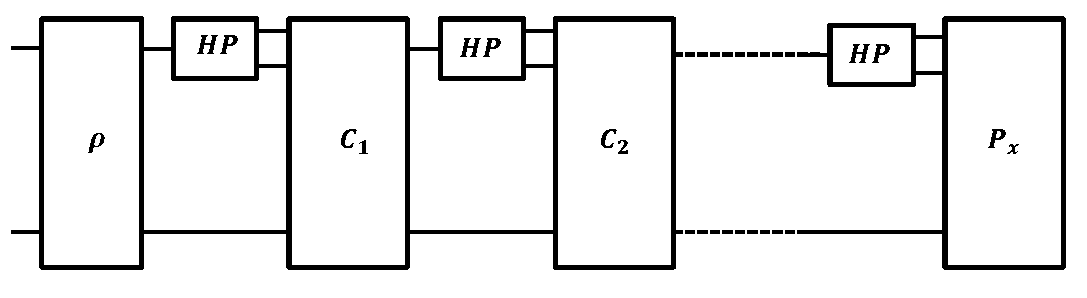
\includegraphics[width=0.6\linewidth]{pics/general-strategy}
		\caption{General strategy}
		\label{circ:cascade-exp}	
	\end{figure}
	\textbf{Description of the above figure:} 
	\begin{itemize}
		\item \textbf{Till $\mathcal{D}_1$:} We prepare an input $A$ of the first use of the process i.e. $\mathcal{C}$ and the other variables are directly def to $\mathcal{D}_1$ then we process again the output of the $\mathcal{C}_1$ with some variables in the lab (untouched ones) at $\mathcal{D}_1$.
		\item \textbf{From $\mathcal{D}_1$ to $\mathcal{D}_2$:} The processed variables at $\mathcal{D}_1$ are then partially fed to the $\mathcal{C}$ and the remaining variables are kept in the lab (untouched).
		\item We keep continuing this till some time and at the end we do \textcolor{red}{observation} which is basically \textbf{a guess on the correct hypothesis} i.e. $\mathcal{P}_x$. $x$ defines the \textbf{correct hypothesis}. The guess \textcolor{red}{$x$ can be either $1$ or $2$ so on and is decided by the number of available prior hypothesis}.
	\end{itemize}
	This is a very general kind of intervention which has \textbf{special cases} in \textit{process tomography}, \textit{parallel strategies} etc.
	\\
	
	\noindent\textbf{NOTE:} The only thing that would not fit in the above framework is when we take into account the ordering of actions i.e. $\mathcal{D}$s the experimentalist considers is \textit{indefinite}
	
	\subsection{Discrimination Rate}
	An important notion when we do an experiment with \textit{finite number of data} is \textbf{how your probability of error or succes depends on the number of experiments you do} which is equivalent to \textbf{how many times you query the black box or the oracle}.
	\\
	
	\begin{itemize}
	\item At the end of the cascaded experiment (check the circuit [\ref{circ:cascade-exp}]) we are going to get a guess on the correct hypothesis and we would like to minimze the \textit{probability of error} i.e. probability of choosing the wrong hypothesis as much as possible.
	\\
	
	\item \textbf{As we do not know what is the causal structure i.e the relation between different variables under consideration so we are going to take a wrost case approach}. Under this consdieration we choose \textbf{\textcolor{red}{worst-case error probability}}
	\begin{equation}
		\mathbf{P}_\text{err}(\mathbf{N}),
	\end{equation} 
	as a function of number of times we probe the black box i.e. $\mathbf{N}$.

	\item \textcolor{red}{$\mathbf{N}$ is very large then the rate at which the $\mathbf{P}_\text{err}(\mathbf{N})$ goes to zero is the most important factor.} It is easy to show that the $\mathbf{P}_\text{err}(\mathbf{N})$ will indeed go to zero. \textbf{This will reach to zero \textit{exponetially} fast, as this is what happens when we do statistics over $\mathbf{N}$ times}. Hence
	\item We want to see \textbf{what is the exponential rate of the decay of the error} which in turns defined as follows
	\begin{equation}
		\frac{-\text{log}\mathbf{P}_\text{err}(\mathbf{N})}{\mathbf{N}},\nonumber
	\end{equation}
	as per probability theory. In the limit $\mathbf{N}\rightarrow\infty$ we get the \textcolor{red}{quantifier of the distinguishibality between the available hypothesis} as follows
	\begin{equation}
		\mathbf{\textcolor{red}{R}} = \lim_{\mathbf{N}\rightarrow\infty} \frac{-\text{log}\;\mathbf{P}_\text{err}(\mathbf{N})}{\mathbf{N}}.
	\end{equation}
	\end{itemize}

\section{Causal Intermediary Identification}
To be noted here we are basically considering \textbf{complete causal intermediary}. Which means \textcolor{red}{$B$ is a causal intermediary of $A$ if all the influences on $A$ must propagate through $B$}.
\begin{figure}[tbh!]
	\centering
	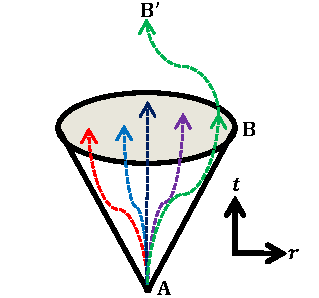
\includegraphics[width=0.3\linewidth]{pics/intermediary}
	\caption{Causal intermediary}
	\label{fig:causal-intermediaty}
\end{figure}
In the spacetime picture we can explain the Fig.[\ref{fig:causal-intermediaty}] as follows
\begin{itemize}
	\item $\mathbf{A}$ is the point which is localized in \textit{spacetime}
	\item The \textit{causal intermediary} $\mathbf{B}$ is \textit{localized in time} but \textit{captures a section in space} i.e. \textbf{A section on the \textit{lightcone} going out from variable $\mathbf{A}$}.
	\item $\mathbf{A}$ can influence another variable $\mathbf{B^\prime}$ which should be mediated by $\mathbf{B}$.
	\item \textbf{More formally:}
	\begin{itemize}
		\item $\mathbf{B}$ is an effect of $\mathbf{A}$.
		\item The whole process from $\mathbf{A}$ to $\mathbf{B^\prime}$ can be decomposed into as process as follows
		\begin{equation}
			\mathbf{A}\rightarrow\mathbf{B}\rightarrow\mathbf{B^\prime}
		\end{equation}
	\end{itemize}
\end{itemize}
\subsection{Exampler Hypothesis on Intermediary}
For variables $A$, $B$ and $C$
\begin{itemize}
	\item \textcolor{red}{1st hypothesis} $B$ is a \textit{causal intermediary} of $A$, where $C$ \textit{\textbf{fluctuates uniform randomly}}
	\item \textcolor{red}{2nd hypothesis} $C$ is a \textit{\textbf{fluctuates uniform randomly}} of $A$, where $B$ \textit{fluctuates uniform randomly}.
\end{itemize}
\textbf{Find out the correct hypothesis}.
\subsubsection{CLASSICAL SOLUTION}
Assume that \textbf{the random variables $A$, $B$ and $C$ have the \textcolor{red}{same dimension d}}. This assumption makes the two hypothesis very simple as follows
\begin{itemize}
	\item \textcolor{red}{1st hypothesis} $b$ (value of variable $B$) is a \textit{\textbf{permutation}} of $a$ (value of variable $A$), where $c$ (value of variable $C$) \textit{fluctuates uniform randomly}
	\item \textcolor{red}{2nd hypothesis} $c$ is a \textit{\textbf{permutation}} of $a$, where $b$ \textit{fluctuates uniform randomly}.
\end{itemize}
\noindent\textbf{\textcolor{red}{Naive strategy}} is to initialize the known variable lets say $A=(000\ldots \lor 111\ldots)$. The advantage of this initialization is that the value that is permutation of $A$ will always have the same value as $A$ and the value that is random at some point will deviate from the $A$ with \textit{high-probability}. Then we repeat the experiment $\mathbf{N}$ times.
\begin{table}[tbh!]
	\centering
\begin{tabular}{lllll}
	& 1 & 2 & 3 & 4 \\ \cline{1-1}
	\multicolumn{1}{|l|}{\textbf{A}} & 0 & 0 & 1 & 1 \\ \cline{1-1}
	\multicolumn{1}{|l|}{\textbf{B}} & 1 & 1 & 0 & 0 \\ \cline{1-1}
	\multicolumn{1}{|l|}{\textbf{C}} & 0 & 0 & 0 & 0 \\ \cline{1-1}
	\end{tabular}
\caption{An example for $\mathbf{N}=5$, $d=2$.}

\label{tab:simple-example-intermediary}
\end{table}
In the the exampler table [\ref{tab:simple-example-intermediary}] we see that $B$ suppose to be the \textit{bit-flip} of $A$ and $C$ is the \textit{identity} but in the \textbf{4th row} it deviates. \textbf{\textcolor{red}{$C$ is the fake effect and $B$ is the true one}}. So if \textbf{we are unlucky} we get $\mathbf{P}_\text{err}(\mathbf{N})=1/2$. If we try $v$ different values of $A$ then the probability of being \textbf{unlucky}
\begin{align}
	\mathbf{P}_\text{unlucky} &= \frac{\text{Number of injective functions from set of $v$ values to a set of $d$ values}}{d^\mathcal{N}}\\
	&=\frac{d(d-1)(d-2)...(d-v-1)}{d^\mathbf{N}}.
\end{align}
In the above case the best thing we can do is to test just one value i.e. $v=1$ then we will have
\begin{equation}
	\mathbf{P}_\text{unlucky}=\frac{d}{d^\mathbf{N}}
\end{equation}
\\

\noindent\textbf{\textcolor{red}{Discrimination rate for $v=1$}} is given by 
\begin{align}
	&\mathbf{P}_\text{err}(\mathbf{N})=\frac{\mathbf{P}_\text{unlucky}}{2}=\frac{1}{2d^{\mathbf{N}-1}}\nonumber\\
	& \mathbf{\textcolor{red}{R}} = \lim_{\mathbf{N}\rightarrow\infty}\frac{-\text{log}\;\mathbf{P}_\text{err}(\mathbf{N})}{\mathbf{N}}\nonumber\\
	& \mathbf{\textcolor{red}{R}}=\text{log}\;d.
\end{align} 
\\

\noindent\textbf{\textcolor{red}{Conclusion}} We do not need to consider the most general strategies but \textbf{the best} we can do is to put the channels in parallel and we can prove that \textbf{asymptotically there is no classical strategy that is better than the naive classical strategy}.

\subsubsection{QUANTUM SOLUTION}
Once again we start with the assumption that $A$, $B$ and $C$ are of same dimension $d$. By considering this the two becomes
\begin{itemize}
	\item \textcolor{red}{1st hypothesis} $\mathcal{C}_{A\rightarrow BC}(\rho_A) = (U\rho U^\dagger)_B\otimes\left(\frac{I}{d}\right)_C$, $U$ is some unknown unitary. Which can be explained as follows. The channel from $A$ to $BC$ should be \textit{Unitary channel} from $A$ to $B$ and some \textit{maximally mixed state on} $C$.
	\item \textcolor{red}{2nd hypothesis} $\mathcal{C}_{A\rightarrow BC}(\rho_A) = \left(\frac{I}{d}\right)_B \otimes (V\rho V^\dagger)_Cs $, $V$ is some unknown unitary. Which can be explained as follows. The channel from $A$ to $BC$ should be \textit{Unitary channel} from $A$ to $C$ and some \textit{maximally mixed state on} $B$.
\end{itemize}
The naive quantum strategy
\begin{figure}[tbh!]
	\centering
	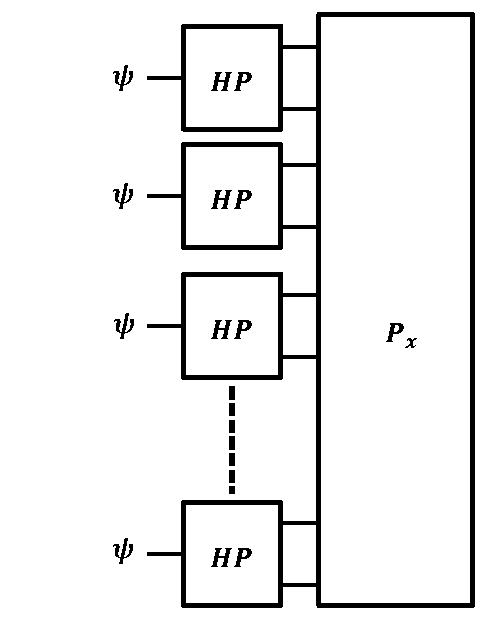
\includegraphics[width=0.5\linewidth]{pics/parallel-strategy}
	\caption{Parallel strategy.}
	\label{circ:naive-quantum-strategy}
\end{figure}
If we use naive quantum strategy as shown in Fig.[\ref{circ:naive-quantum-strategy}] then we get an error probability
\begin{equation}
	\mathbf{P}_\text{err}=\frac{\binom{\mathbf{N}+d-1}{d-1}}{2d^\mathbf{N}}
\end{equation}
which is \textbf{worst than the classical} but at least the \textbf{discrimination rate} is
\begin{equation}
	\text{log}\;d
\end{equation}
\\
\textbf{\textcolor{red}{Full Tomography of the Channel}} which is illustrated in the \textbf{Figure [\ref{circ:quantum-strategy-tomography}]}. We prepare a correlated system $\Psi$ of the input variable $A$ together with some reference system $R$ in a fixed state, repeating it $\mathbf{N}$ times, and then measuring the output state.
\begin{figure}[tbh!]
	\centering
	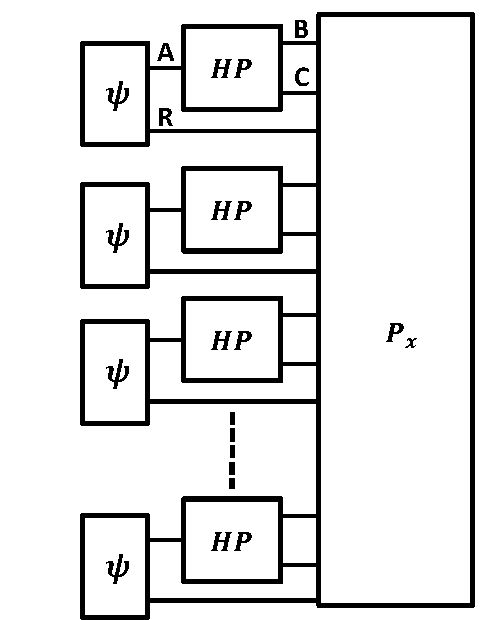
\includegraphics[width=0.5\linewidth]{pics/parallel-strategy-tomography}
	\caption{Complete tmography of the quantum channel.}
	\label{circ:quantum-strategy-tomography}
\end{figure}
this also give us the same \textcolor{red}{discrimination rate} of
\begin{equation}
	\text{log}\;d
\end{equation}
\\
\textbf{\textcolor{red}{Parallel Strategies}}
Previously we had the \textbf{initialization} in such a way that the input state was of the following form $\mathbf{\Psi} \otimes\mathbf{\Psi}\otimes\mathbf{\Psi}\otimes\mathbf{\Psi}\cdots\otimes\mathbf{\Psi}$ so there was \textcolor{red}{correlation inbetween the inputs}. In the current strategy \textcolor{red}{we will allow correlation in the initialization} without a reference state as depicted in \textbf{Figure [\ref{circ:parallel-strategy-without-reference}]} and with a reference system as depicted in \textbf{Figure [\ref{circ:parallel-strategy-with-reference}]}
\begin{figure}
	\centering
	\begin{minipage}{0.45\textwidth}
		\centering
		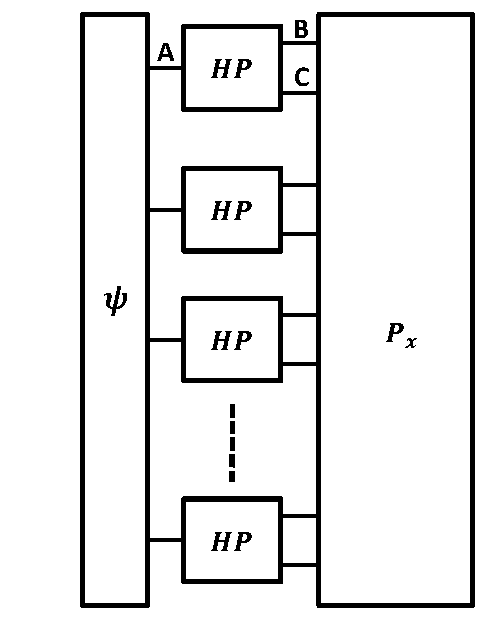
\includegraphics[width=0.9\textwidth]{pics/parallel-strategy-without-reference}
		\caption{Without reference.}
		\label{circ:parallel-strategy-without-reference}
	\end{minipage}\hfill
	\begin{minipage}{0.45\textwidth}
		\centering
		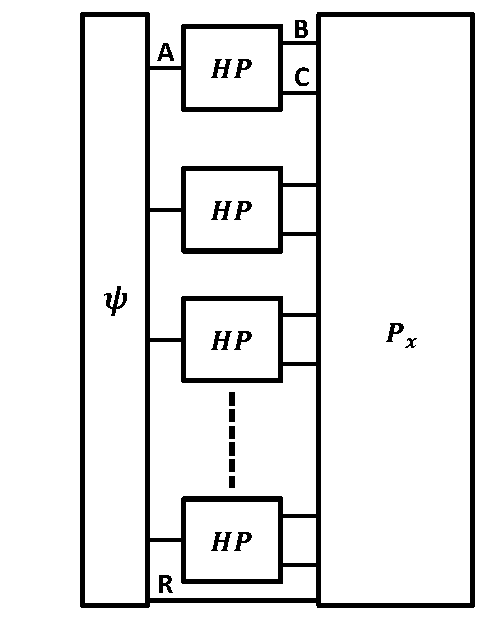
\includegraphics[width=0.9\textwidth]{pics/parallel-strategy-with-reference}
		\caption{With reference.}
		\label{circ:parallel-strategy-with-reference}
	\end{minipage}
\end{figure}
The main motivation behind analysing the \textit{without reference} and \textit{with reference} scenerio is that \textbf{the without reference case is more general hence the solution of this setting will give us a better understanding of the outcomes in with reference settings}
\\

\textbf{\textcolor{red}{Parallel Strategy without reference}} the \textbf{optimal} strategy is to assume $d=2$ and $\mathbf{N}$ is even say $\mathbf{N}=2p$ so that \textbf{we can divide the $\mathbf{N}$ input variables in the groups of two and then to initialize each pair in a singlet state}
\begin{equation}
	|\Psi\rangle = \frac{ |0 \rangle \otimes 1 \rangle - 1 \rangle \otimes 0 \rangle }{\sqrt{2}}
\end{equation}
The reason behind initializing in singlet is the fact that \textbf{the singlet state is invarient under Unitary changes of basis} i.e. 
\begin{equation}
	U\otimes U |\Psi\rangle = |\Psi\rangle
\end{equation}
hence \textbf{we get rid of that we do not know the functional dependency between the cause and effect by choosing a quantum state that is entangled and by removing that dependency i.e we can test the causal structure by not knowing the fucntional dependency between cause and effect}. For a general dimention $d$, we divide the $\mathcal{N}$ input variables in groups of $d$ and prepare each group in the following sinlget
\begin{equation}
	|S_d\rangle = \frac{1}{\sqrt{d!}}\sum_{a_1,a_2,\cdots,k_d}^{}\epsilon_{a_1,a_2,\cdots,a_d}  |a_1\rangle|a_2\rangle\cdots|a_d\rangle
\end{equation}
then we get an error probability
\begin{equation}
	\mathbf{P}_\text{err}(\mathbf{N})=\frac{1}{2d^\mathbf{N}}
\end{equation}
which is better than the classical $\frac{1}{2d^{\mathbf{N}-1}}$ dependence but the discrimination rate is still
\begin{equation}
	\text{log}\; d,
\end{equation}
\\

\textbf{\textcolor{red}{Parallel Strategy with reference}} in this case we choose $d=2$, just like the case above, $\mathbf{N}$ is once again even. And there are many ways to partition the inputs into pairs as depicted in \textbf{Figure \ref{circ:partition}}
\begin{figure}
	\centering
	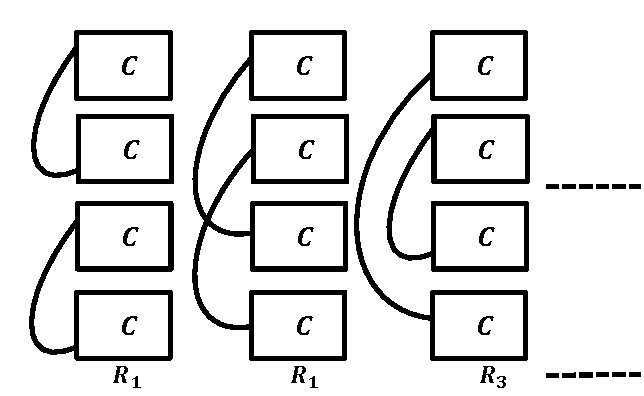
\includegraphics[width=0.6\linewidth]{pics/equivalent-strategy}
	\caption{Many ways to partition with corresponding reference system.}
	\label{circ:partition}
\end{figure}
\textbf{We can associate different reference states to different partition configutation and suporpose them} which practically means we are creating an \textbf{entangled state} where we \textbf{entangle the reference system with the partition configuration of the system} as follows
\begin{equation}
	|\Psi\rangle = \frac{1}{\sqrt{L}}\sum_{i=1}^{L}\left(|S_d\rangle^{\otimes \mathbf{N}/d}\right)_i\otimes|i\rangle_R.
\end{equation}
$i$ defines the possible ways of grouping the systems and $L$ is the number of groupings in superposition. If there are $r$ linearly independent groupings then the error probability becomes
\begin{equation}
	\mathbf{P}_\text{err}(r) = \frac{r}{2d^\mathcal{N}}\left(1-\sqrt{1-r^{-2}}\right)\rightarrow\left[\frac{1}{4rd^\mathbf{N}}\right]_{r\gg1},
\end{equation}
picking the maximum $r$ we obtain the \textbf{discrimination rate}
\begin{equation}
	\mathbf{\textcolor{red}{R_Q}} = -\lim_{\mathbf{N}\rightarrow\infty}\frac{\text{log}\;\mathbf{P}_\text{err}}{\mathbf{N}}=2\text{log}\;d
\end{equation}

\section{Conclusion}
The \textbf{general quantum strategy} uses the \textbf{fidelity divergence} method to get the divergence in quantum states from each other when two quantum channels representing the two hypothesis are considered. Then the \textbf{general strategy} actually upperbounds the discrimination rate that is
\begin{equation}
	\textcolor{red}{\mathbf{P}^\text{general}_{Q}} \leq 2\text{log}\;d
\end{equation} 
\textcolor{red}{Asymptotically the best quantum discrimination rate is $2\text{log}\; d$}.
\end{document}